\section{Background}
\label{sec:background}

% Homepage2Vec
\textbf{Homepage2Vec}~\cite{homepage2vec} is a multilingual website topic classification model capable of providing embeddings for websites in any language. 

The model is trained on the publicly available website directory called Curlie~\textit{CITE}, maintained by a volunteer community. The directory comprises three million websites in 92 languages, following a taxonomy of hierarchical topics. After removing duplicates and retaining accessible sites, the dataset contained 886K entries. For classification, only top-level labels were considered, resulting in 14 classes. The label distribution is imbalanced, with most websites categorised as Business (27\%), Society (13.9\%) and Arts (9\%). In contrast, the lowest represented classes are Home (1.5\%), News (1.1\%) and Kids and Teens (1.1\%). The dataset is primarily single-labeled, with only 2.1\% of samples appearing in two or more taxonomy trees of the 14 top-level classes~\cite{homepage2vec}.

Architecturally, Homepage2Vec is an embeddings-based model utilising pre-trained textual extractors to process the various features of a website useful for topic classification. Specifically, the model scrapes a website's homepage, parses the raw HTML, and extracts the \texttt{tld}, \texttt{domain}, \texttt{metatags}, \texttt{title}, \texttt{description}, \texttt{keywords}, \texttt{links}, and \texttt{sentences} as features. With the exception of \texttt{tld} and \texttt{metatags}, which are one-hot encoded, all features are embedded via the multilingual model XLM-R~\cite{xmlr} and finally concatenated, resulting in a website embedding of dimension $4665$. The resulting embedding is then fed into a fully connected neural network with 2 hidden layers of sizes 1000 and 100, respectively, each followed by a ReLU activation function and dropout with a probability of $0.5$. Importantly, each output logit is a binary classifier for a single category, giving the model the ability to predict multiple labels for a single website by thresholding the output logits. 

\begin{figure}[!ht]
    \centering
    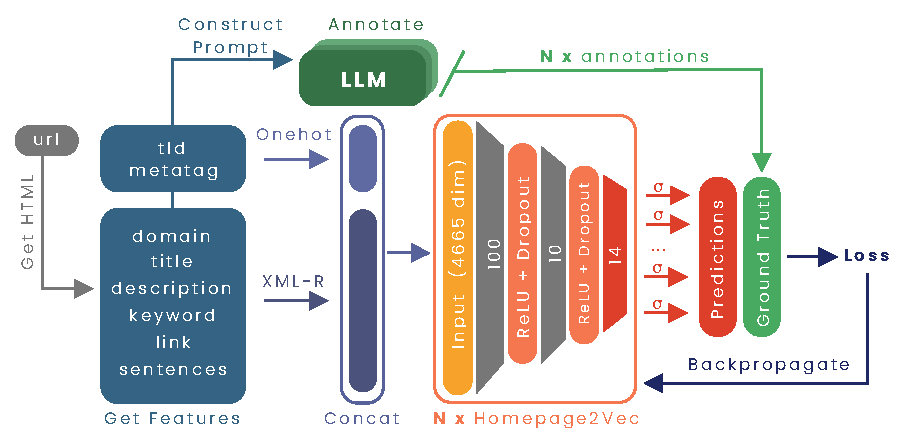
\includegraphics[height=0.2\textheight, width=\columnwidth]{./figures/training_overview.pdf}
    \caption{\textbf{Training overview.} Sth else}
    \label{fig:train-overview}
\end{figure}

Homepage2Vec, evaluated against an unbalanced Curlie test set, achieves a macro-averaged precision of 77.1\%, recall of 54.9\%, and an F1-score of 63.4\%~\cite{homepage2vec}. While these results are promising, they don't overestimate the model's performance as the test data also only contains single-labeled websites. We therefore evaluated the model on the \texttt{crowdsourced} dataset, where each website has an average of $2.5$ labels. We obtain a macro F1-score of $39.16\%$, serving as our baseline for further improvement using the proposed methods described in the following section.

\textbf{LLM Labeling.} Previous studies have demonstrated that LLMs are capable of executing various tasks without being specifically trained for them~\textit{CITE}, especially when providing an informative prompt, a few examples, and a task description. This makes LLMs an attractive candidate to perform website classification directly by simply providing a set of features as input and ask the model to predict from a set of website categories.
However, direct inference using LLMs is less practical due to their substantial cost and time demands during inference. A more better approach is therefore to use LLMs to create a training dataset for a classifier, a technique known as \textit{knowledge distilation}~\textit{CITE} and shown  effective in prior studies~\cite{reduce-labeling-cost, prompt-tuning, is-gpt3-good-annot, annollm}. Contrasting with earlier research that concentrated on single-label classification with limited categories, our research explores the quality of LLM-generated labels in a more complex scenario of multi-label classification across 14 website topics.
